\documentclass [a4paper, 11pt] {article}

%document configuration
\newcommand{\courseName}{Machine Learning in Graphics \& Vision}
\newcommand{\termYear}{Summer Term 2020}
\newcommand{\homeworkNum}{3}
\newcommand{\studentOne}{Driton Goxhufi}
\newcommand{\studentTwo} {Damir Ravlija}
\newcommand{\matrikelNrStOne}{4233242}
\newcommand{\matrikelNrStTwo}{5503184}
\newcommand{\mailStOne}{driton.goxhufi@student.uni-tuebingen.de}
\newcommand{\mailStTwo}{damir.ravlija@student.uni-tuebingen.de}

%packages
\usepackage [english] {babel}
\usepackage [T1] {fontenc}
\usepackage [utf8] {inputenc}
\usepackage {graphicx}
\usepackage {subcaption}
\usepackage {amsmath}
\usepackage {amssymb}
\usepackage {amstext}
\usepackage {amsthm}
\usepackage {listings}
\usepackage {tikz}
\usepackage[
pdftex,
pdfauthor={Goxhufi, Driton; Ravlija, Damir},
pdftitle={MLGV - Exercise \homeworkNum Submission},
pdfsubject={Machine Learning in Graphics \& Vision Homework}
]{hyperref}

\usepackage[a4paper,lmargin={2cm},rmargin={2cm},tmargin={3.5cm},bmargin = {2.5cm},headheight = {4cm}]{geometry}

\usepackage[shortlabels]{enumitem}
\usepackage{lastpage}
\usepackage{fancyhdr}

\usepackage{lipsum}
\usepackage{ifthen}

\pagestyle{fancy}



%other config
\renewcommand{\v}[1]{\boldsymbol{#1}}
\newcommand{\mat}[1]{\boldsymbol{#1}}
\newcommand{\m}[1]{\begin{pmatrix}#1\end{pmatrix}}
\newcommand{\tr}[2]{{}^{#1}T_{#2}}
\graphicspath{{./images/}}


\lhead{\begin{tabular}{l}
		\courseName\\
		\termYear \\
		Exercise \homeworkNum
\end{tabular}}
\rhead{\begin{tabular}{lr}
		\studentOne & \matrikelNrStOne \\
		\studentTwo & \matrikelNrStTwo \\
\end{tabular}}

\begin{document}
	
\title{\vspace{-1.5cm}\textbf{Exercise \homeworkNum} \\ 
	\courseName}
\author{\begin{tabular}{lcr}
		\studentOne & \matrikelNrStOne & \href{mailto:\mailStOne}{\mailStOne} \\
		\studentTwo & \matrikelNrStTwo & \href{mailto:\mailStTwo}{\mailStTwo} 
\end{tabular}}	
\date{}
\maketitle


\section{Task 1}
\begin{enumerate}
\item[(a)]
Our implementation does achieve 97.05\% accuracy after 15 epochs.\\
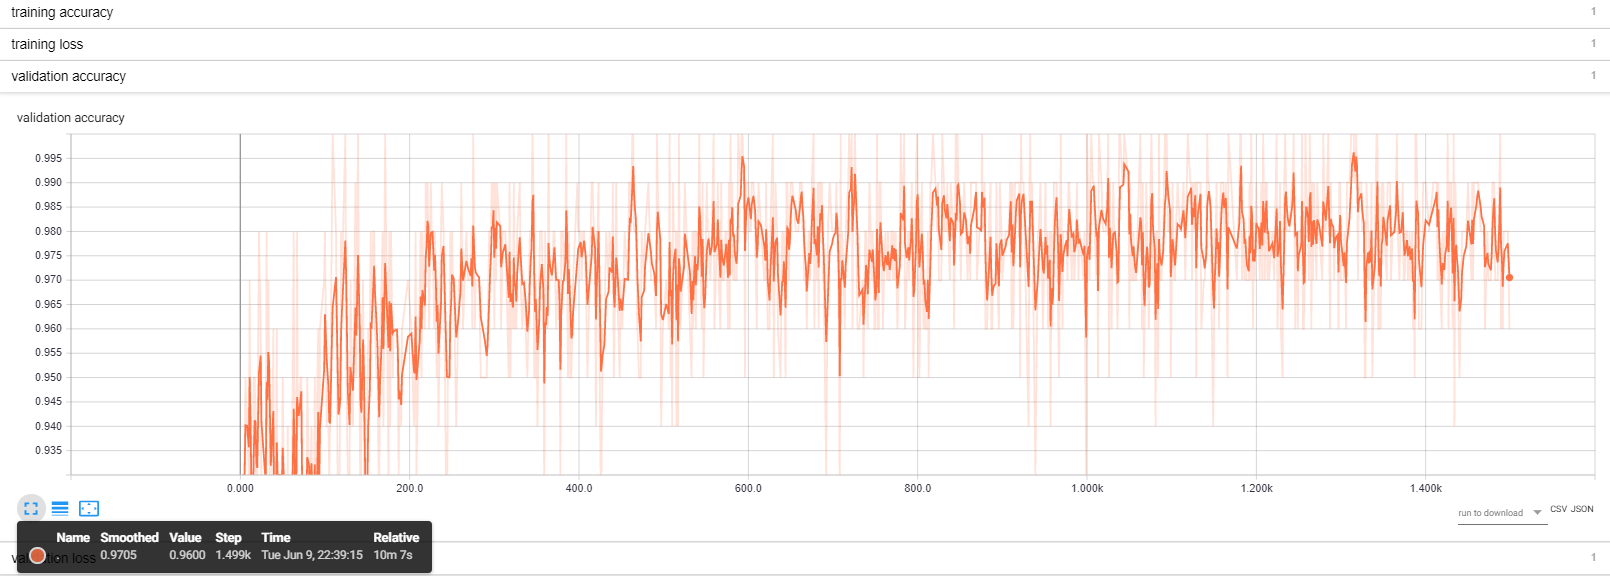
\includegraphics{img/validation_acc_15epochs.png}\\
According to \url{http://rodrigob.github.io/are_we_there_yet/build/classification_datasets_results.html#4d4e495354} the paper "Regularization of Neural Networks using DropConnect" in 2013 achieved a result of 0.21\% errorrate, hence an accuracy value of 99.79\%.

\item[(b)]
from torchsummary import summary\\
summary(model, (1,28,28))\\
----------------------------------------------------------------\\
Layer (type)               Output Shape         Param \#\\
==========================\\
Conv2d-1           [-1, 32, 28, 28]             320\\
ReLU-2           [-1, 32, 28, 28]               0\\
Conv2d-3           [-1, 32, 28, 28]           9,248\\
ReLU-4           [-1, 32, 28, 28]               0\\
Conv2d-5           [-1, 32, 28, 28]           9,248\\
Linear-6                  [-1, 256]       6,422,784\\
ReLU-7                  [-1, 256]               0\\
Linear-8                   [-1, 10]           2,570\\
==========================\\
Total params: 6,444,170\\
Trainable params: 6,444,170\\
Non-trainable params: 0\\
----------------------------------------------------------------\\
Input size (MB): 0.00\\
Forward/backward pass size (MB): 0.96\\
Params size (MB): 24.58\\
Estimated Total Size (MB): 25.55\\
----------------------------------------------------------------\\

Output of convolutional layers can be calculated with this formula: 

\begin{align*}
\left[(W-K+2P)/S\right]+1 \\
\end{align*}

where $W$ is the width(or height if the input is squared), $K$ is the kernelsize, $P$ is the amount of padding and $S$ the stride.

\item[(c)]
After 15 epochs training on the default network with FashionMNIST dataset, \\
the validation(test) accuracy is about 89\%.\\
Console output:\\
epoch done:  14
accuracy train 0.9082844034830729
accuracy test 0.891600112915039\\
\\
After tweaking (hyper)parameters of the network: 
% TODO:
\item[(d)]

\end{enumerate}
	
\end{document}

